%\VignetteEngine{knitr}
%\VignetteIndexEntry{HUPO 2014 pRoloc poster}
%\VignetteKeywords{bioinformatics, spatial proteomics, mass spectrometry}

\documentclass[final]{beamer}\usepackage[]{graphicx}\usepackage[]{color}
%% maxwidth is the original width if it is less than linewidth
%% otherwise use linewidth (to make sure the graphics do not exceed the margin)
\makeatletter
\def\maxwidth{ %
  \ifdim\Gin@nat@width>\linewidth
    \linewidth
  \else
    \Gin@nat@width
  \fi
}
\makeatother

\definecolor{fgcolor}{rgb}{0.345, 0.345, 0.345}
\newcommand{\hlnum}[1]{\textcolor[rgb]{0.686,0.059,0.569}{#1}}%
\newcommand{\hlstr}[1]{\textcolor[rgb]{0.192,0.494,0.8}{#1}}%
\newcommand{\hlcom}[1]{\textcolor[rgb]{0.678,0.584,0.686}{\textit{#1}}}%
\newcommand{\hlopt}[1]{\textcolor[rgb]{0,0,0}{#1}}%
\newcommand{\hlstd}[1]{\textcolor[rgb]{0.345,0.345,0.345}{#1}}%
\newcommand{\hlkwa}[1]{\textcolor[rgb]{0.161,0.373,0.58}{\textbf{#1}}}%
\newcommand{\hlkwb}[1]{\textcolor[rgb]{0.69,0.353,0.396}{#1}}%
\newcommand{\hlkwc}[1]{\textcolor[rgb]{0.333,0.667,0.333}{#1}}%
\newcommand{\hlkwd}[1]{\textcolor[rgb]{0.737,0.353,0.396}{\textbf{#1}}}%

\usepackage{framed}
\makeatletter
\newenvironment{kframe}{%
 \def\at@end@of@kframe{}%
 \ifinner\ifhmode%
  \def\at@end@of@kframe{\end{minipage}}%
  \begin{minipage}{\columnwidth}%
 \fi\fi%
 \def\FrameCommand##1{\hskip\@totalleftmargin \hskip-\fboxsep
 \colorbox{shadecolor}{##1}\hskip-\fboxsep
     % There is no \\@totalrightmargin, so:
     \hskip-\linewidth \hskip-\@totalleftmargin \hskip\columnwidth}%
 \MakeFramed {\advance\hsize-\width
   \@totalleftmargin\z@ \linewidth\hsize
   \@setminipage}}%
 {\par\unskip\endMakeFramed%
 \at@end@of@kframe}
\makeatother

\definecolor{shadecolor}{rgb}{.97, .97, .97}
\definecolor{messagecolor}{rgb}{0, 0, 0}
\definecolor{warningcolor}{rgb}{1, 0, 1}
\definecolor{errorcolor}{rgb}{1, 0, 0}
\newenvironment{knitrout}{}{} % an empty environment to be redefined in TeX

\usepackage{alltt} 

\mode<presentation> {  %% check http://www-i6.informatik.rwth-aachen.de/~dreuw/latexbeamerposter.php for examples
  %% \usetheme{CCP}
}

% footline colors and fonts
\setbeamercolor{footline}{fg=white,bg=gray}
\setbeamerfont{footline}{fg=black,size=\normalsize}

\setbeamertemplate{footline}{
  \begin{beamercolorbox}[wd=\paperwidth]{upper separation line foot}
    \rule{0pt}{2pt}
  \end{beamercolorbox}
  \leavevmode%
  \begin{beamercolorbox}[ht=2ex]{footline}%
    \centering
    HUPO meeting
    \hskip3ex 
    5 -- 8 October 2014
    \hskip3ex 
    Madrid
  \end{beamercolorbox}
  \vskip0pt%
  \begin{beamercolorbox}[wd=\paperwidth]{lower separation line foot}
    \rule{0pt}{2pt}
  \end{beamercolorbox}
}


\setbeamertemplate{bibliography item}[text]

\boldmath
\usepackage[orientation=portrait,size=a0,scale=1.4,debug]{beamerposter}                        % e.g. for DIN-A0 poster
%\usepackage[orientation=portrait,size=a1,scale=1.4,grid,debug]{beamerposter}                  % e.g. for DIN-A1 poster, with optional grid and debug output
%\usepackage[size=custom,width=200,height=120,scale=2,debug]{beamerposter}                     % e.g. for custom size poster
%\usepackage[orientation=portrait,size=a0,scale=1.0,printer=rwth-glossy-uv.df]{beamerposter}   % e.g. for DIN-A0 poster with rwth-glossy-uv printer check
% ...
%

%% hide navigation symbols (bottom right)
\setbeamertemplate{navigation symbols}{}

\usepackage{lipsum}
\usepackage{ragged2e} 
\usepackage[english]{babel}
\usepackage[latin1]{inputenc}
\usepackage{amsmath,amsthm, amssymb, latexsym}
\usefonttheme[onlymath]{serif}

\usepackage{graphicx}
\usepackage{caption}
\usepackage{subcaption}

\usepackage{tcolorbox}
\usepackage{changepage} %% provided adjustwidth
\usepackage{framed}

\newenvironment{Leftbar}{%
  \def\FrameCommand{\vrule width 3pt \hspace{20pt}}%
  \MakeFramed {\advance\hsize-\width \FrameRestore}}%
 {\endMakeFramed}

\newcommand{\R}{\texttt{R} }
\newcommand{\code}[1]{{\texttt{#1}}}
\newcommand{\Rfunction}[1]{{\texttt{#1}}}
\newcommand{\Robject}[1]{{\texttt{#1}}}
\newcommand{\Rpackage}[1]{{\mbox{\texttt{#1}}}}
\newcommand{\email}[1]{\href{mailto:#1}{\normalfont\texttt{#1}}}

\newcommand{\challenge}[1]{
       \begin{tcolorbox}[notitle,boxrule=1pt,colback=blue!10,colframe=blue!25]
         {#1}
       \end{tcolorbox}
}

\newcommand{\secintro}[1]{
  \bigskip
  \begin{tcolorbox}[notitle,boxrule=0pt,colback=blue!10,colframe=blue!10]{#1}\end{tcolorbox}}


%% colors
\definecolor{Red}{rgb}{0.7,0,0}
\definecolor{Blue}{rgb}{0,0,0.8}


\usepackage[bordercolor=white, backgroundcolor=gray!20]{todonotes}

\usepackage{hyperref}
\usepackage{breakurl}
\hypersetup{%
  pdfauthor={Laurent Gatto},%
  pdfusetitle,
  bookmarks = {true},
  bookmarksnumbered = {true},
  bookmarksopen = {true},
  bookmarksopenlevel = 2,
  unicode = {true},
  breaklinks = {false},
  hyperindex = {true},
  colorlinks = {true},
  linktocpage = {true},
  plainpages = {false},
  linkcolor = {Blue},
  citecolor = {Blue},
  urlcolor = {Red},
  pdfstartview = {Fit},
  pdfpagemode = {UseOutlines},
  pdfview = {XYZ null null null}
}



%% figure numering
\usecaptiontemplate{ 
  \small 
  \structure{\insertcaptionname~\insertcaptionnumber:} 
  \insertcaption 
} 

\title[pRoloc]{\huge A state-of-the-art machine learning pipeline for the\\
  analysis of spatial proteomics data}

\author[Gatto et al.]{
  \large Laurent Gatto$^{1,2,*}$, Lisa M. Breckels$^{1,2}$, Thomas Naake$^{1,2}$,\\ Samuel Wieczorek$^{3}$, Thomas Burger$^{3}$, Kathryn S. Lilley$^{2}$
}

\institute[CPU]{
  \begin{small}
    $^{1}$Computational Proteomics Unit and $^{2}$Cambridge Centre for Proteomics, Department of Biochemistry, University of Cambridge, UK \\
    $^{3}$Universit/'e Grenoble-Alpes, CEA (iRSTV/BGE), INSERM (U1038), CNRS (FR3425), 38054 Grenoble, France \\
    \bigskip
    $^{*}$\url{lg390@cam.ac.uk} \hspace{5cm}  \url{http://cpu.sysbiol.cam.ac.uk}
  \end{small}
}




\date[HUPO 2014]{HUPO Meeting, 5 -- 8 October 2014}
\date[]{}
\IfFileExists{upquote.sty}{\usepackage{upquote}}{}
\begin{document}


%%$

\begin{frame}[fragile]

  \maketitle

  \begin{columns}
    \begin{column}{.48\textwidth}
      \challenge{
        \begin{block}{Introduction}     
          \vspace{3mm}
          \begin{large}
            \Rpackage{pRoloc} and \Rpackage{pRolocGUI} are
            \texttt{R}/Bioconductor packages that implement all the
            necessary tools for the sound and reproducible analysis
            and interactive exploration of spatial proteomics data
            from any type of experiment.
            \end{large}

          \bigskip 

          \begin{large}
            Below, we illustrate a typical \Rpackage{pRoloc} analysis
            pipeline: \justifying
            \begin{enumerate}
            \item Loading data into \texttt{R} and adding markers
            \item QC: checking resolution in the data and organelle
              markers
            \item Detection of new organelle clusters
            \item Classification of unlabelled proteins
            \item Results, interpretation and visualisation
            \end{enumerate}            
          \end{large}
        \end{block}
       }
     

     % \vspace{2cm}
       \vfill

      \begin{block}{1) Data input}

        We start by reading quantitative data from 10 fractions (at
        positions 2 to 11 in the data spreadsheet) sampled along a
        separation gradient from a \texttt{csv} file and add
        \textit{Drosophila} organelle markers. This code creates an
        \Robject{MSnSet} data object (named \Robject{spat}) that
        stores the quantitative data and the metadata, and can
        subsequently be easily manipulated, plotted and further
        processed.

\begin{knitrout}
\definecolor{shadecolor}{rgb}{0.969, 0.969, 0.969}\color{fgcolor}\begin{kframe}
\begin{alltt}
\hlstd{spat} \hlkwb{<-} \hlkwd{readMSnSet2}\hlstd{(}\hlstr{"quant-data.csv"}\hlstd{,} \hlkwc{ecols} \hlstd{=} \hlnum{2}\hlopt{:}\hlnum{11}\hlstd{)}
\hlstd{spat} \hlkwb{<-} \hlkwd{addMarkers}\hlstd{(spat,} \hlstr{"dmel"}\hlstd{)}
\end{alltt}
\end{kframe}
\end{knitrout}
      \end{block}
      \begin{figure}
        \centering
        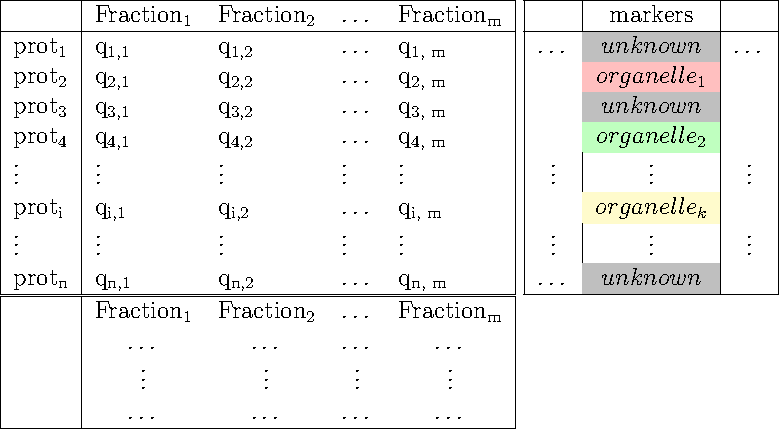
\includegraphics[width=.75\linewidth]{./figures/Fig1-data-a.pdf}
      \end{figure}
      \bigskip

      \begin{block}{2) Quality control}

        We verify on a PCA plot that there is structure in the data
        (i.e we distinguish well defined clusters, left) and that the
        markers defined well resolved organelle clusters (right).

\begin{knitrout}
\definecolor{shadecolor}{rgb}{0.969, 0.969, 0.969}\color{fgcolor}\begin{kframe}
\begin{alltt}
\hlkwd{plot2D}\hlstd{(spat)}
\hlkwd{addLegend}\hlstd{(spat)}
\end{alltt}
\end{kframe}
\end{knitrout}

      \end{block}
      \begin{figure}
        \centering
        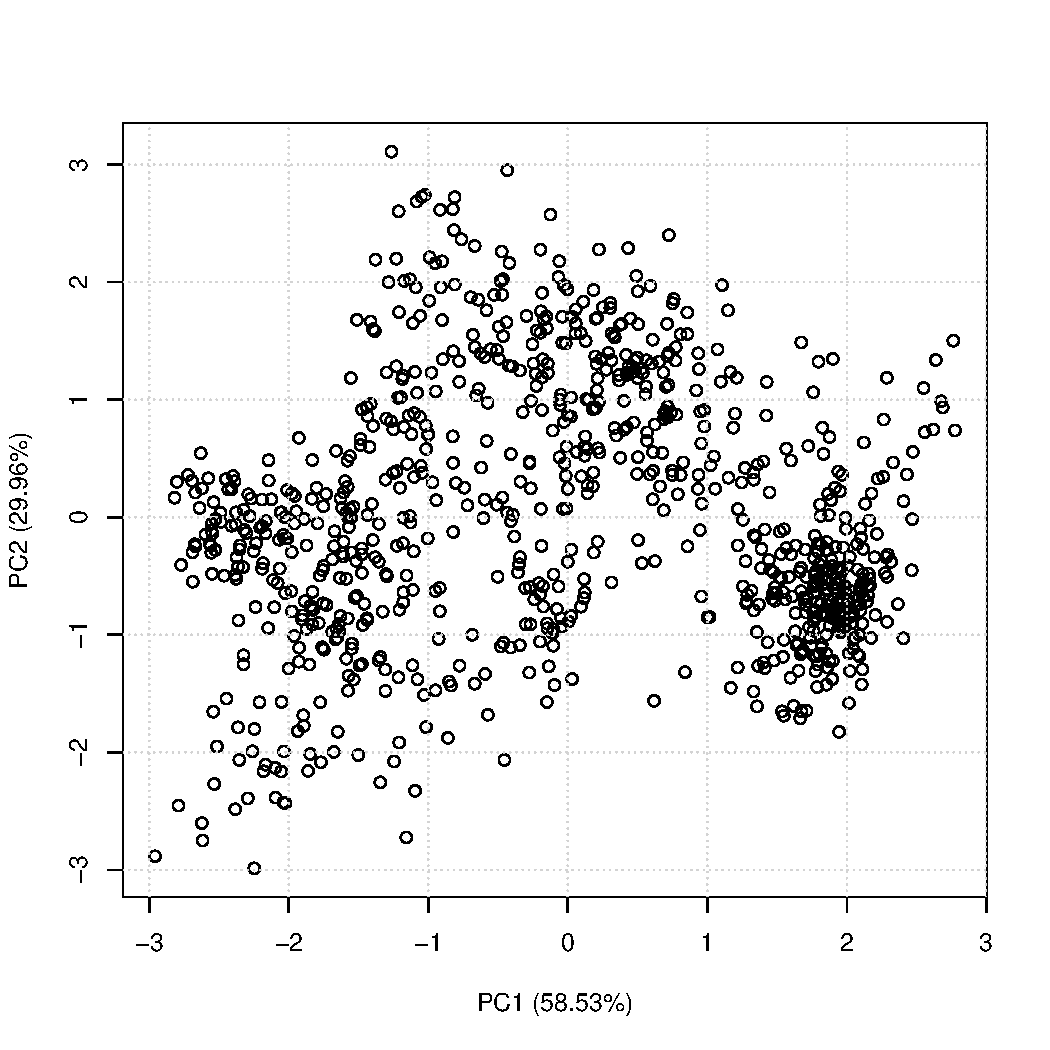
\includegraphics[width=.49\linewidth]{./figures/pca1.pdf}
        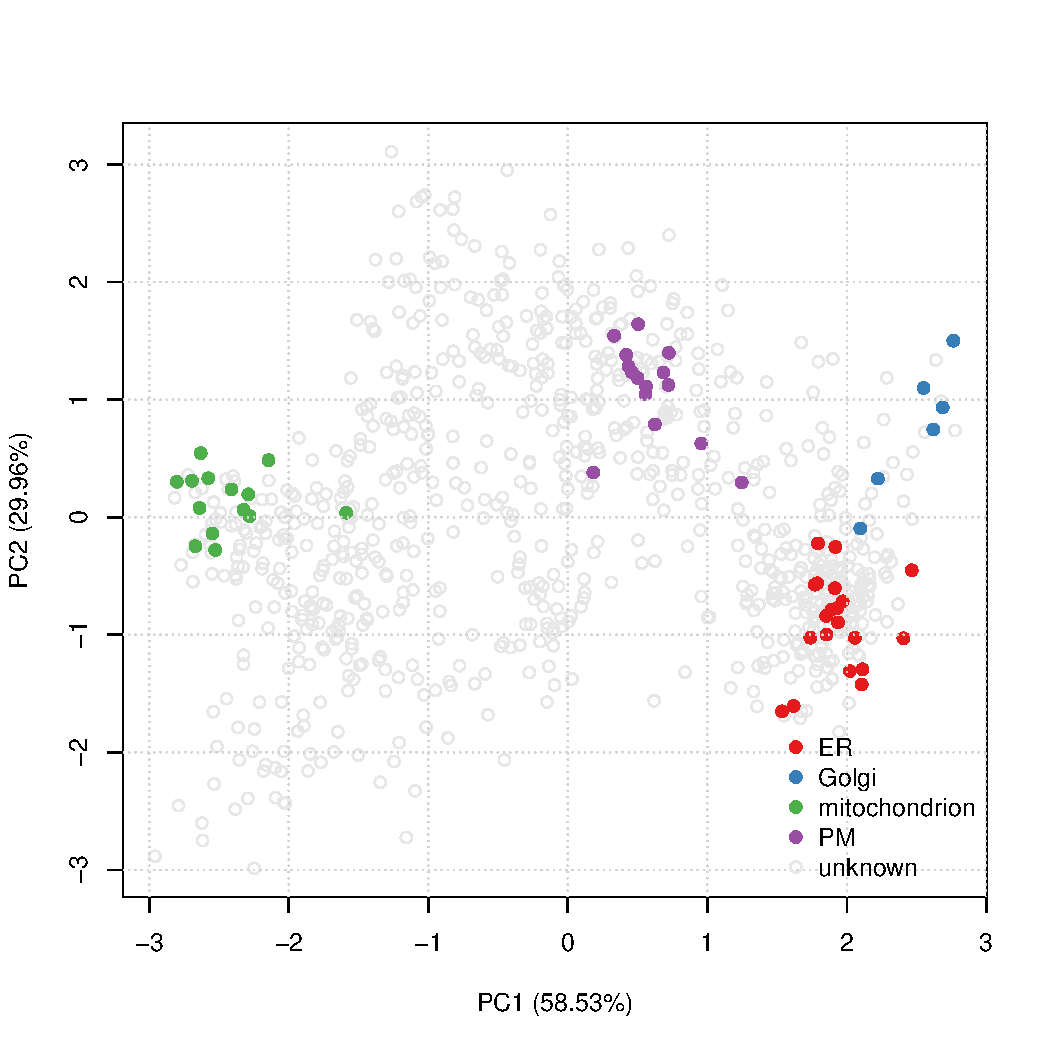
\includegraphics[width=.49\linewidth]{./figures/pca2.pdf}
      \end{figure}


      \challenge{        
        Gatto \textit{et al.} \emph{Mass-spectrometry-based spatial
          proteomics data analysis using pRoloc and pRolocdata.}
        Bioinformatics. 2014 May 1;30(9):1322-4. PMID: 24413670.

        \noindent Gatto \textit{et al.}  \emph{A foundation for
          reliable spatial proteomics data analysis.}  Mol Cell
        Proteomics. 2014 Aug;13(8):1937-52. PMID: 24846987.

        \vspace{2mm}
        \begin{description}
        \item[software] \url{http://is.gd/pRoloc}
        \item[documentation] \url{http://is.gd/pRoloc_tutorial}
        \item[GUI] \url{http://is.gd/pRolocGUI}
        \item[data] \url{http://is.gd/pRolocdata}  
        \end{description}
        \vspace{2mm}
    }

    \end{column}

    \begin{column}{.48\textwidth}  

      \begin{block}{3) Novelty detection}
        
        Our manually curated markers do not cover the entire
        sub-cellular diversity. We use a semi-supervised machine
        learning algorithms to identify new putative organelle
        clusters, called \emph{phenotypes} (left), which require
        validation by the user (right).

\begin{knitrout}
\definecolor{shadecolor}{rgb}{0.969, 0.969, 0.969}\color{fgcolor}\begin{kframe}
\begin{alltt}
\hlstd{spat} \hlkwb{<-} \hlkwd{phenoDisco}\hlstd{(spat)}
\hlkwd{plot2D}\hlstd{(spat,} \hlkwc{fcol} \hlstd{=} \hlstr{"pd"}\hlstd{)}
\end{alltt}
\end{kframe}
\end{knitrout}

      \begin{figure}
        \centering
        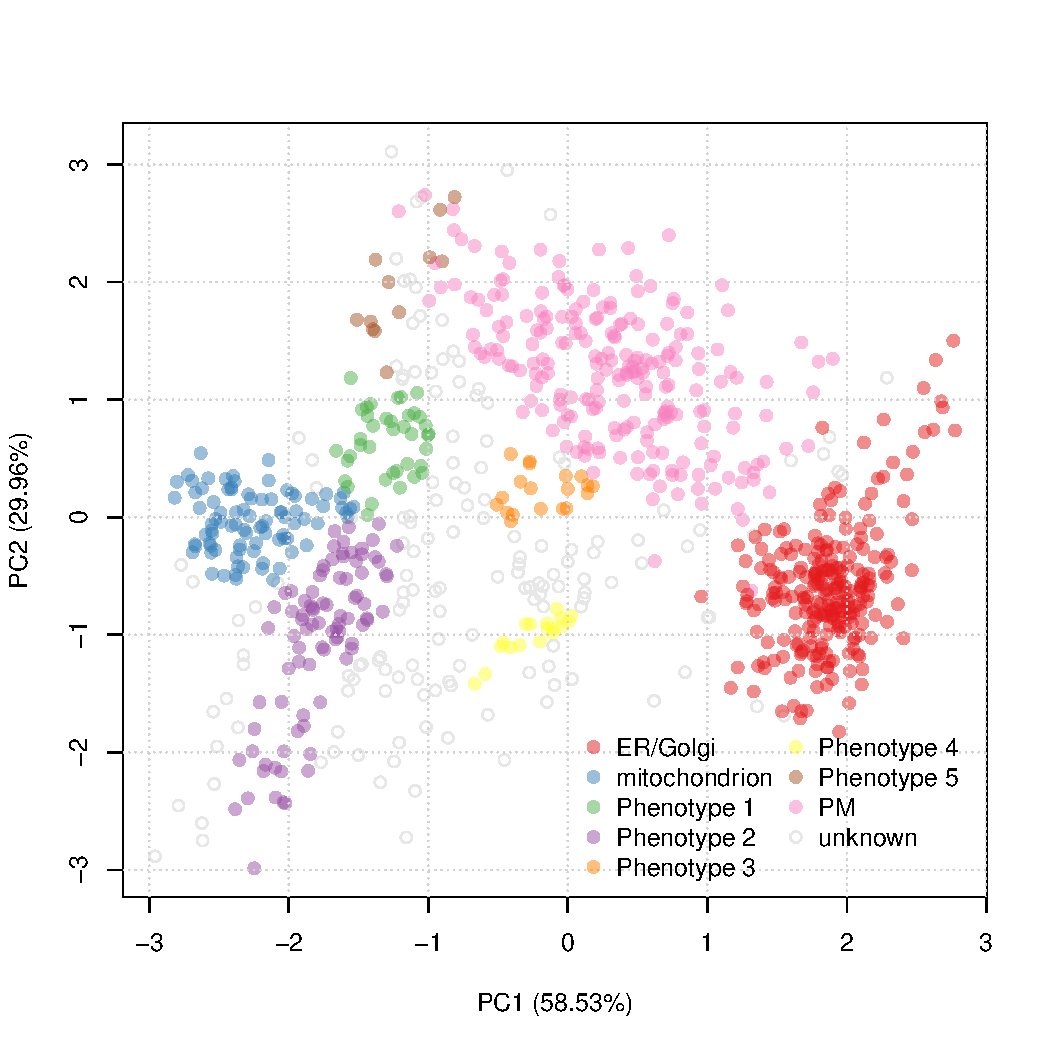
\includegraphics[width=.41\linewidth]{./figures/pca3.pdf}
        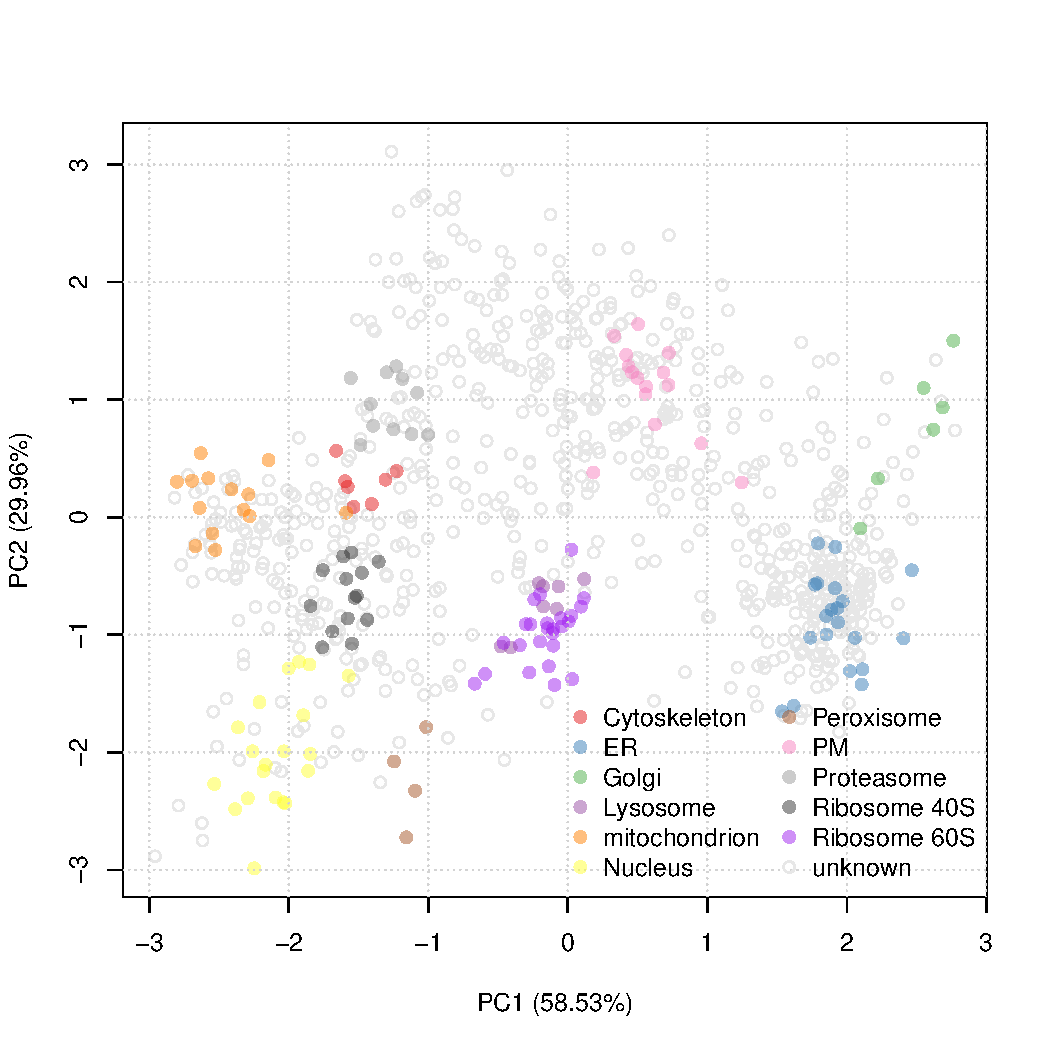
\includegraphics[width=.41\linewidth]{./figures/pca4.pdf}
      \end{figure}

      \end{block}
      \begin{block}{4) Classification}

        We can now classify unlabelled proteins to any of the
        augmented classes using a supervised machine (SVM) learning
        algorithms, for example, a support vector machine
        classifier. It is essential to tune the classification model
        parameters (here $sigma$ and $cost$) prior to actual
        classification (left).

\begin{knitrout}
\definecolor{shadecolor}{rgb}{0.969, 0.969, 0.969}\color{fgcolor}\begin{kframe}
\begin{alltt}
\hlstd{params} \hlkwb{<-} \hlkwd{svmOptimisation}\hlstd{(spat,} \hlkwc{fcol} \hlstd{=} \hlstr{"pd.markers"}\hlstd{)}
\hlstd{spat} \hlkwb{<-} \hlkwd{svmClassification}\hlstd{(spat, params,} \hlkwc{fcol} \hlstd{=} \hlstr{"pd.markers"}\hlstd{)}
\end{alltt}
\end{kframe}
\end{knitrout}

The classification algorithm calculates classification probabilities
that reflect the distance of a protein to the decision boundaries
defined by the SVM model (right). Eventually, the data can be exported
to a spreadsheet file.
        
\begin{knitrout}
\definecolor{shadecolor}{rgb}{0.969, 0.969, 0.969}\color{fgcolor}\begin{kframe}
\begin{alltt}
\hlstd{ptsze} \hlkwb{<-} \hlkwd{exp}\hlstd{(}\hlkwd{fData}\hlstd{(spat)}\hlopt{$}\hlstd{svm.scores)} \hlopt{-} \hlnum{1}
\hlkwd{plot2D}\hlstd{(spat,} \hlkwc{fcol} \hlstd{=} \hlstr{"svm"}\hlstd{,} \hlkwc{cex} \hlstd{= ptsze)}
\hlkwd{write.exprs}\hlstd{(spat,} \hlkwc{file} \hlstd{=} \hlstr{"spat-results.csv"}\hlstd{)}
\end{alltt}
\end{kframe}
\end{knitrout}

      \end{block}
        

\begin{figure}[ht]
  \begin{minipage}[t]{0.45\textwidth}
    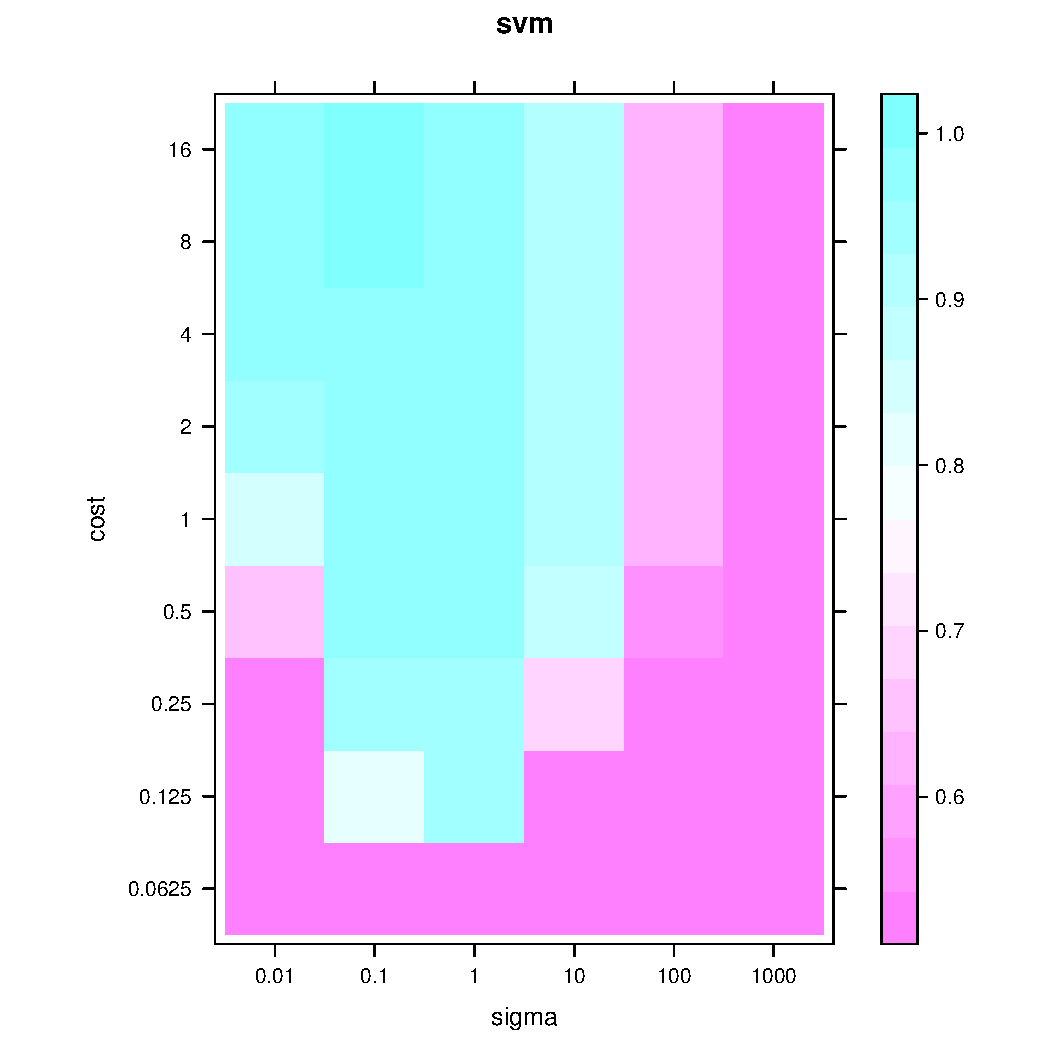
\includegraphics[width=1\textwidth]{./figures/opt1.pdf}
  \end{minipage}
  \hfill
  \begin{minipage}[t]{0.53\textwidth}
    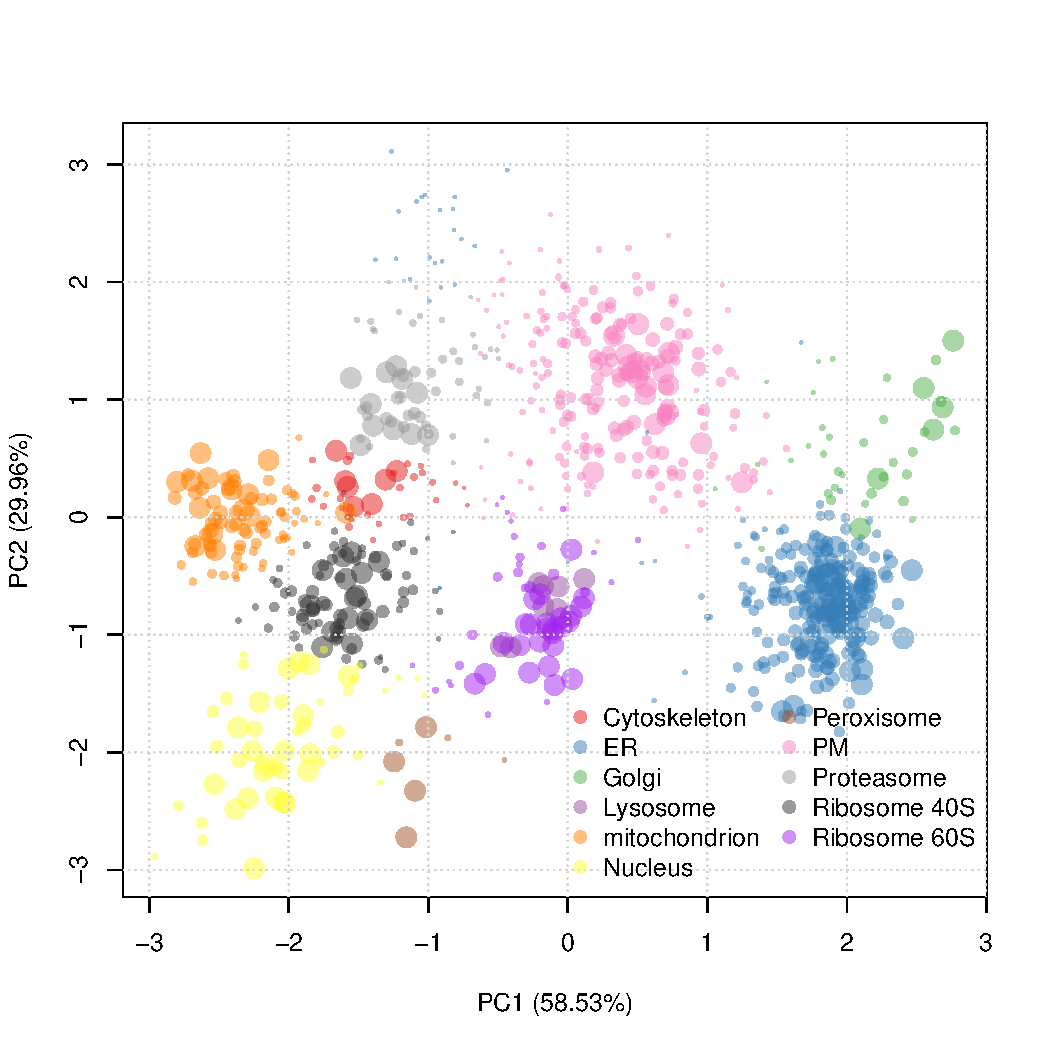
\includegraphics{./figures/svm.pdf}
  \end{minipage}
\end{figure}

      % \begin{figure}
      %   \centering
      %   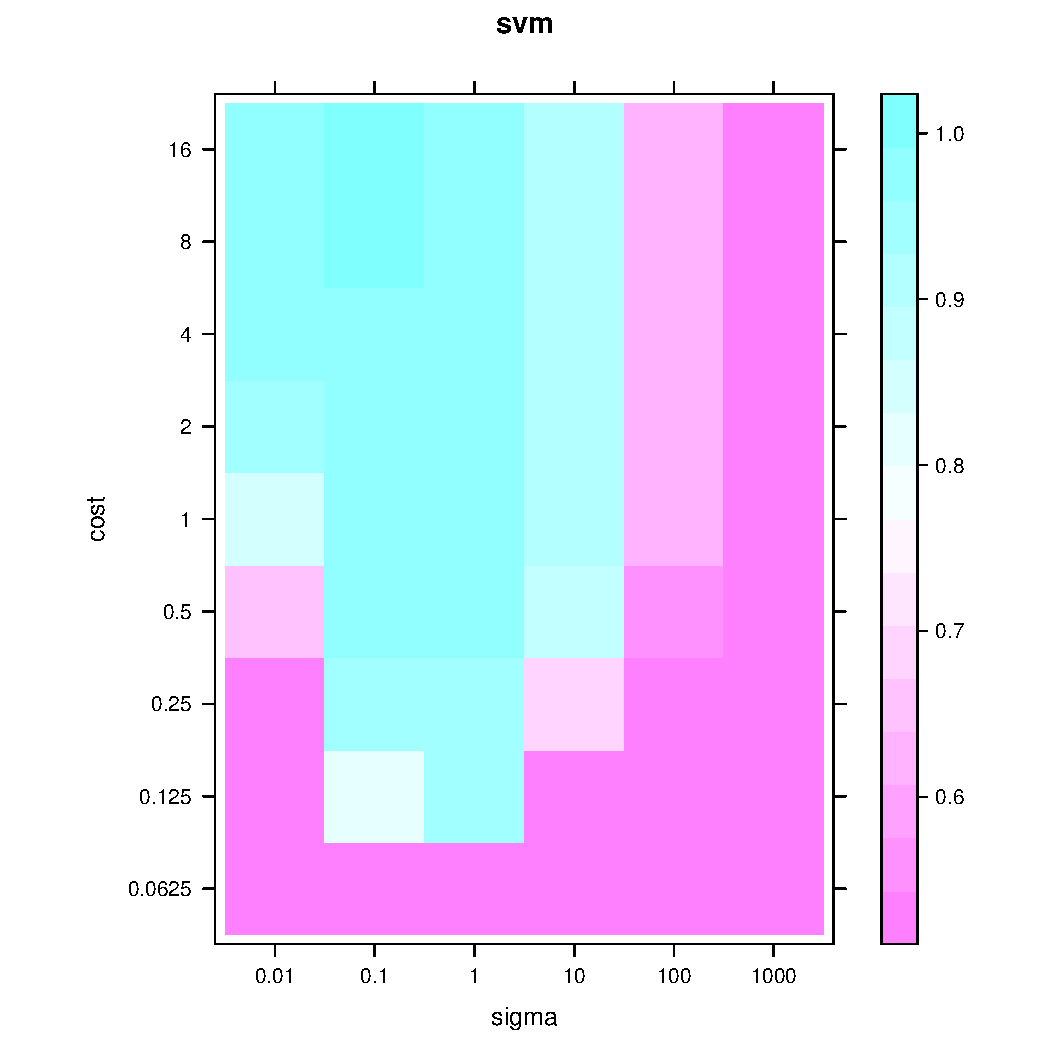
\includegraphics[width=.3\linewidth]{./figures/opt1.pdf}
      %   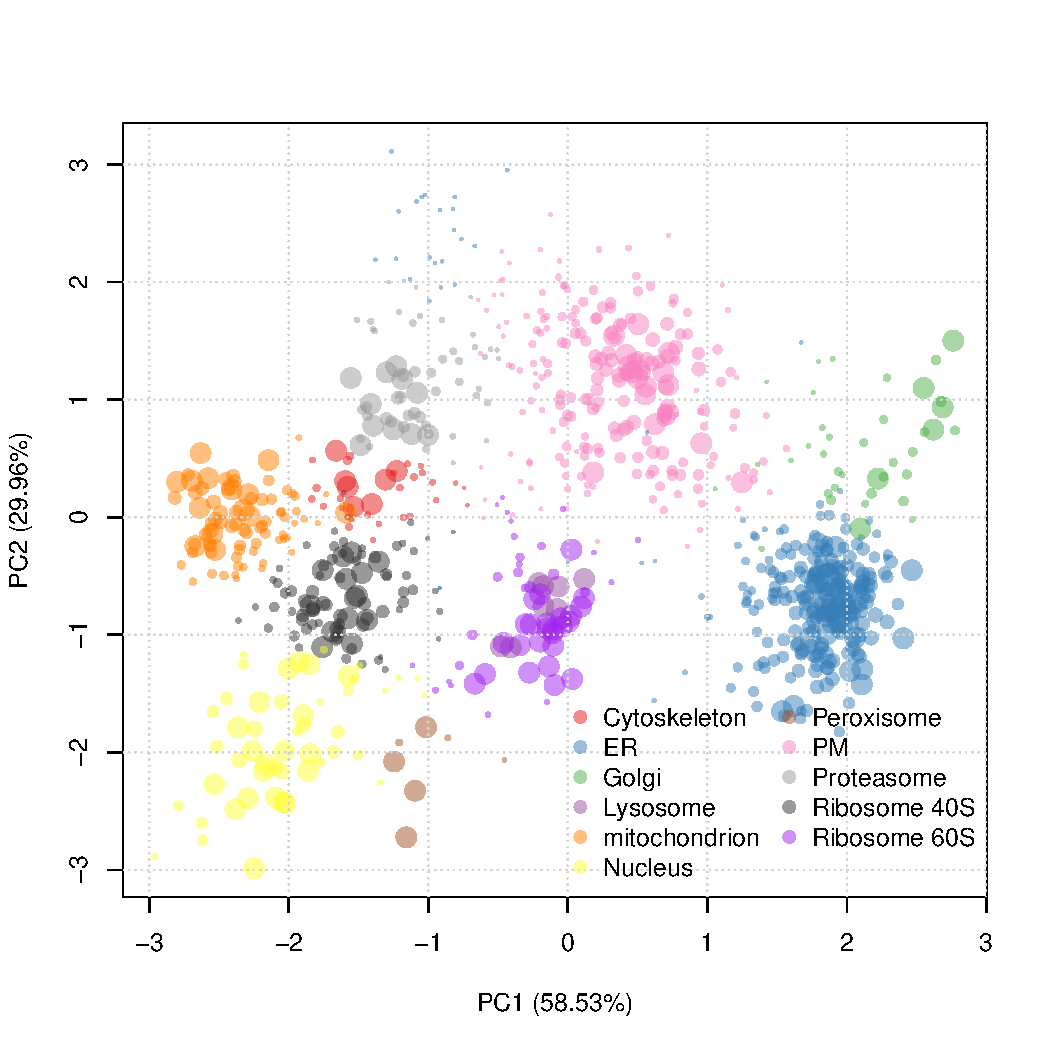
\includegraphics[width=.49\linewidth]{./figures/svm.pdf}
      % \end{figure}

      \begin{block}{5) Interpretation}
        The graphical user interface implemented in the
        \Rpackage{pRolocGUI} package enables one the interactively
        explore the data.
\begin{knitrout}
\definecolor{shadecolor}{rgb}{0.969, 0.969, 0.969}\color{fgcolor}\begin{kframe}
\begin{alltt}
\hlkwd{library}\hlstd{(}\hlstr{"pRolocGUI"}\hlstd{)}
\hlkwd{pRolocVis}\hlstd{(spat)}
\end{alltt}
\end{kframe}
\end{knitrout}
      \end{block}
      \begin{figure}
        \centering
        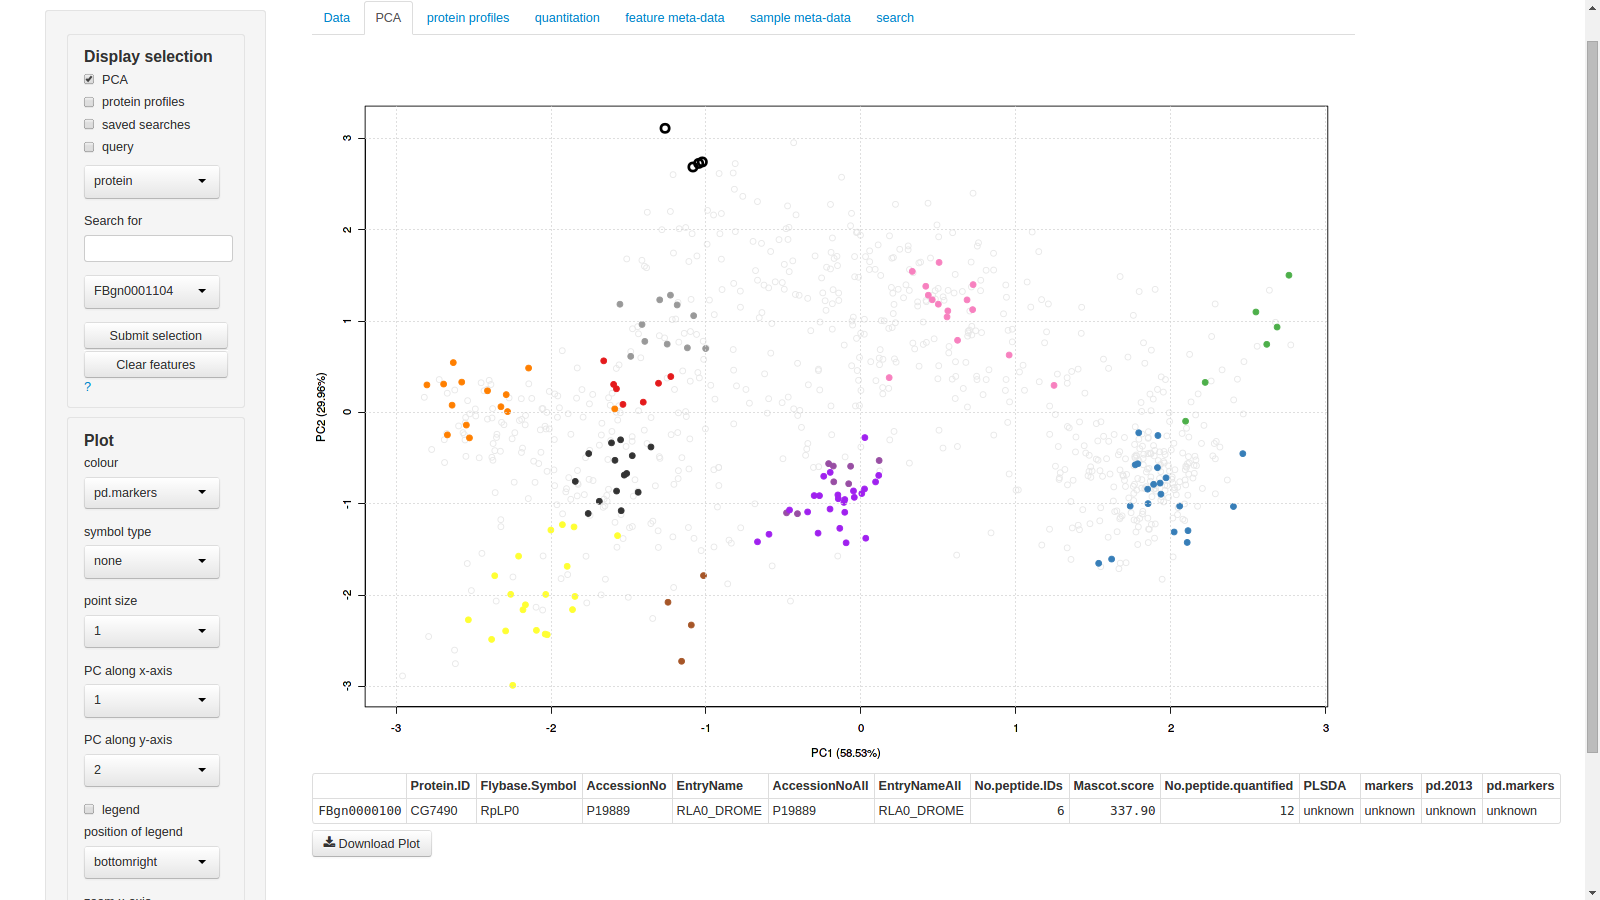
\includegraphics[width=.5\linewidth]{./figures/gui1.png}
        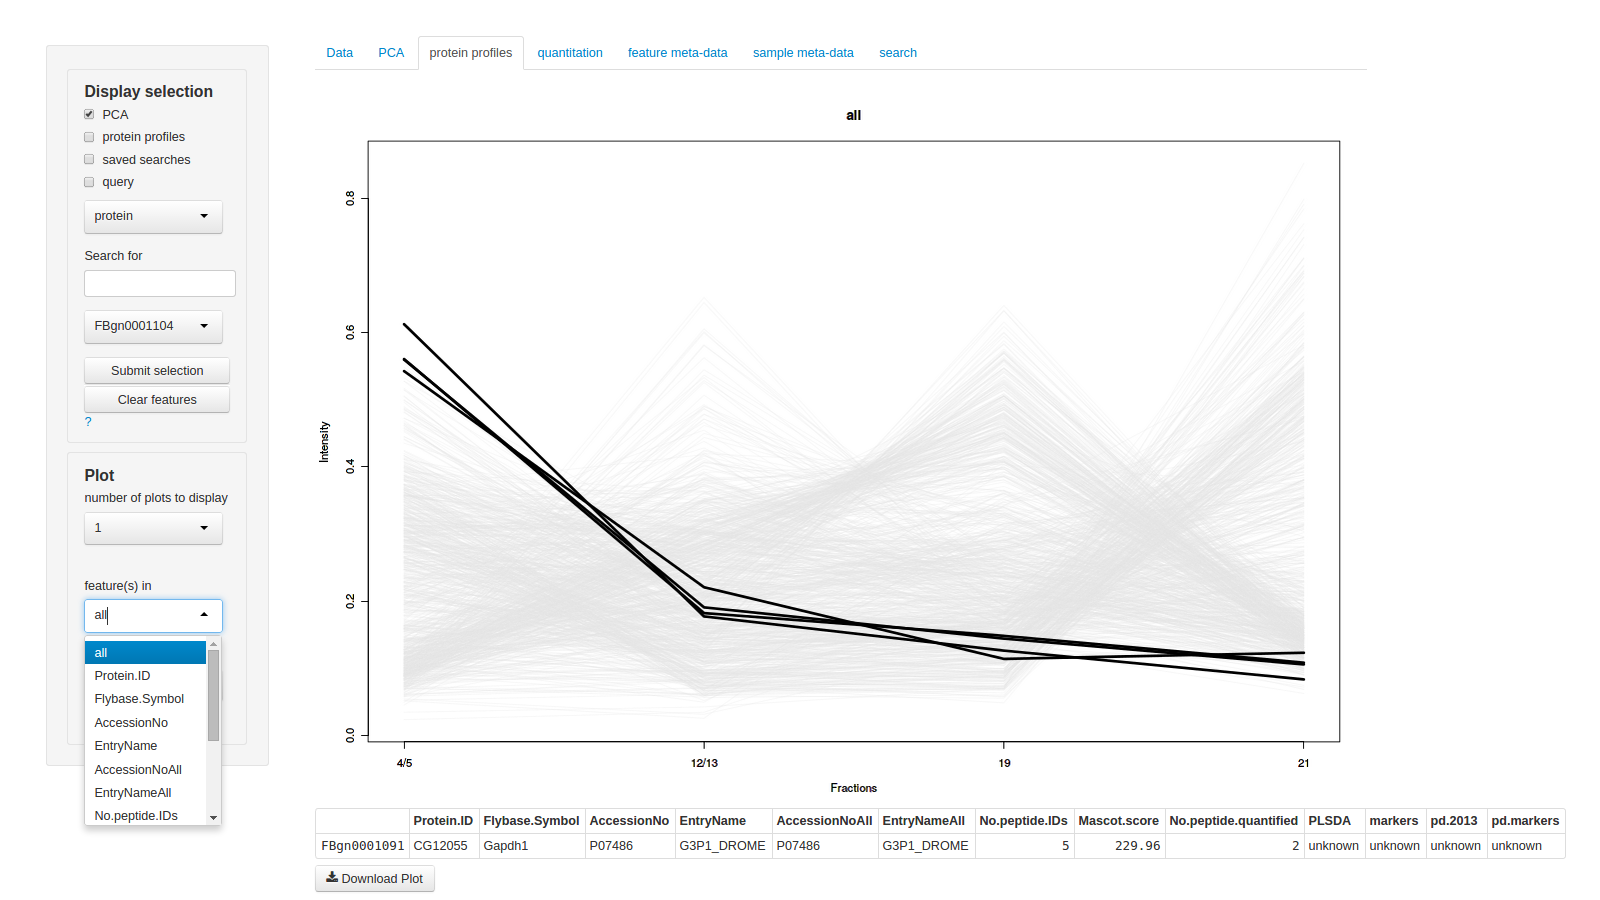
\includegraphics[width=.5\linewidth]{./figures/gui2.png}
      \end{figure}

      {\small This work was supported by the \textbf{European Union
          7$^{th}$ Framework Program PRIME-XS project} and a
        \textbf{BBSRC Tools and Resources Development Fund}.}

    \end{column}    
  \end{columns}
\end{frame}

\end{document}

